\section{Description and Methodology}

\subsection{Linux build process}
To build the uCLinux distribution for the microcontroller, PTXDist is
used\cite{ptxdistguru}. This is done because the features of a real
distribution is wanted, and PTXDist allows to create a unique distribution.

\begin{verbatim}
ptxdist select configs/ptxconfig
ptxdist platform <platform>
ptxdist toolchain <toolchain>
\end{verbatim}

\noindent
These commands are run to set the userland configuration, which platform to
develop for and choosing the toolchain to build for this platform

\begin{verbatim}
ptxdist go
\end{verbatim}

\noindent
Is used to compile the components needed. The script is smart enough to not
compile everything every time it is ran, so it can be used to just compile
some parts of the project.

\begin{verbatim}
ptxdist images
\end{verbatim}

\noindent
To build the image that can be flashed to the device, this command is used. To
not build the root image every time other parts of the distribution is edited,
the specific image to build can be used.

\begin{verbatim}
ptxdist test flash-all
\end{verbatim}

\noindent
This is used to flash all images to the device. Again, to not flash things that
don't need to be flashed each time, a more specific image to flash can be given
as argument.


\subsection{The driver}

To receive button inputs from the player, a driver for the provided game pad was
implemented. Because the game pad isn't discoverable, it is implemented as a
platform device. This means that the platform driver\footnotemark registers
that it can handle the device "tdt4259", which is then matched by the system to
the platform device by the same name.

\footnotetext{
  \url{https://www.kernel.org/doc/Documentation/driver-model/platform.txt}
}

As opposed to the old way of implementing drivers in Linux, when the kernel
module is loaded or unloaded, it is merely registered or unregistered as an
available platform driver. The system will then call the registered probe and
remove functions when required, shown in Algorithms~\ref{func:probe}
and~\ref{func:remove} respectively.

When the system calls the probe() function, the module initializes the game pad
hardware, allocates and maps memory to access the game pad's signal lines,
registers the game pad device with sysfs and then creates a character device
which can be read from userspace.

\begin{algorithm}
  \footnotesize
  \caption{Platform driver probe}
  \begin{algorithmic}[1]
    \Function{probe}{pdev}
      \State $\Call{hardware\_init}{\null}$ \\

      \State $irq\_even \gets \Call{platform\_get\_irq}{pdev, irq\_even}$
      \State $irq\_odd \gets \Call{platform\_get\_irq}{pdev, irq\_odd}$
      \State $\Call{request\_irq}{irq\_even, irq\_handler, \
        irqf\_disabled, device\_name, null}$
      \State $\Call{request\_irq}{irq\_odd, irq\_handler, \
        irqf\_disabled, device\_name, null}$ \\

      \State $res \gets \Call{platform\_get\_resource}{pdev,
        ioresource\_mem, 0}$
      \State $size \gets \Call{resource\_size}{res}$
      \State $\Call{request\_mem\_region}{res.start,  size, \
        pdev{\rightarrow}name}$ \\

      \State $cl \gets \Call{class\_create}{this\_module, device\_name}$
      \State $\Call{device\_create}{cl, null, devno, null, device\_name}$ \\

      \State $\Call{alloc\_chrdev\_region}{\&devno, 0, 1, device\_name}$ \\
      \State $\Call{cdev\_init}{\&c\_dev, \&f\_ops}$
      \State $c\_dev.owner \gets this\_module$
      \State $\Call{cdev\_add}{\&c\_dev, devno, 1}$ \\

      \State $\Call{interrupt\_enable}{\null}$
    \EndFunction
  \end{algorithmic}
  \label{func:probe}
\end{algorithm}

When remove() the character device is destroyed, the interrupt handler is
removed and game pad I/O lines are released.
 
\begin{algorithm}[H]
  \footnotesize
  \caption{Platform driver remove}
  \begin{algorithmic}[1]
    \Function{remove}{pdev}
      \State $\Call{interrupt\_disable}{\null}$ \\
      \State $\Call{cdev\_del}{\&c\_dev}$
      \State $\Call{device\_destroy}{c, devno}$
      \State $\Call{unregister\_chrdev\_region}{0, 1}$ \\

      \State $irq\_even \gets \Call{platform\_get\_irq}{pdev, irq\_even}$
      \State $irq\_odd \gets \Call{platform\_get\_irq}{pdev, irq\_odd}$
      \State $\Call{free\_irq}{irq\_even}$
      \State $\Call{free\_irq}{irq\_odd}$ \\

      \State $res \gets \Call{platform\_get\_resource}{pdev, \
        ioresource\_mem, 0}$
      \State $size \gets \Call{resource\_size}{res}$
      \State $\Call{release\_mem\_region}{res.start, size}$
    \EndFunction
  \end{algorithmic}
  \label{func:remove}
\end{algorithm}

When the user presses a button, the button interrupt handler~\ref{func:irq} is
called. This caches the current state of the game pad buttons, and sends a
SIGIO signal to userspace, which can read the state of the gamepad buttons by
calling $read()$ on the character device.

\begin{algorithm}
  \footnotesize
  \caption{Button interrupt handler}
  \begin{algorithmic}[1]
    \Function{irq\_handler}{irq, dev\_id, regs}
      \State $\Call{gpio\_interrupt\_flags\_clear}{\null}$
      \State $button\_state \gets \Call{gpio\_button\_state}{\null}$
      \If {$async\_queue$}
        \State $\Call{kill\_fasync}{\&async\_queue, sigio, poll\_in}$
      \EndIf
    \EndFunction
  \end{algorithmic}
  \label{func:irq}
\end{algorithm}

By using an interrupt to read the gamepad, and a signal to notify userspace,
the presented solution attempts to conserve energy, by sleeping the CPU as much
as possible. By presenting the raw state of the gamepad buttons, as opposed to
passing button events to userspace, applications are offered flexibility in how
to handle button presses, whether that be caching the state internally, as is
done here, or by generating button events in userspace.

\subsection{The game}

The game implemented is Pong. Focus during development was kept on keeping code
clean and maintainable, using correct game programming patterns whenever
possible, while still keeping focus on energy efficiency.

The game was designed with stubs for IO and display,
allowing local development via the game library allegro \cite{allegro}.
This greatly sped up development, as compile times were reduced to a minimum.

As Pong is a 'real time' game, the amount of time one can spend asleep is
somewhat reduced compared to a game like chess,
where the game can be entirely gamepad interrupt driven.

Additional care is taken to redraw the minimum amount of pixels necessary
during screen updates, as system calls take valuable CPU cycles not available.
Heavy calculations such as collision detection are avoided until the last
minute possible.

To conserve power, the game enters sleep mode after rendering a frame,
allowing for a very high rate of sleep
($ 94\% $ with a framerate of $ 60 $ and a render time of $ 1 ms $).

\begin{figure}[H]
\centering
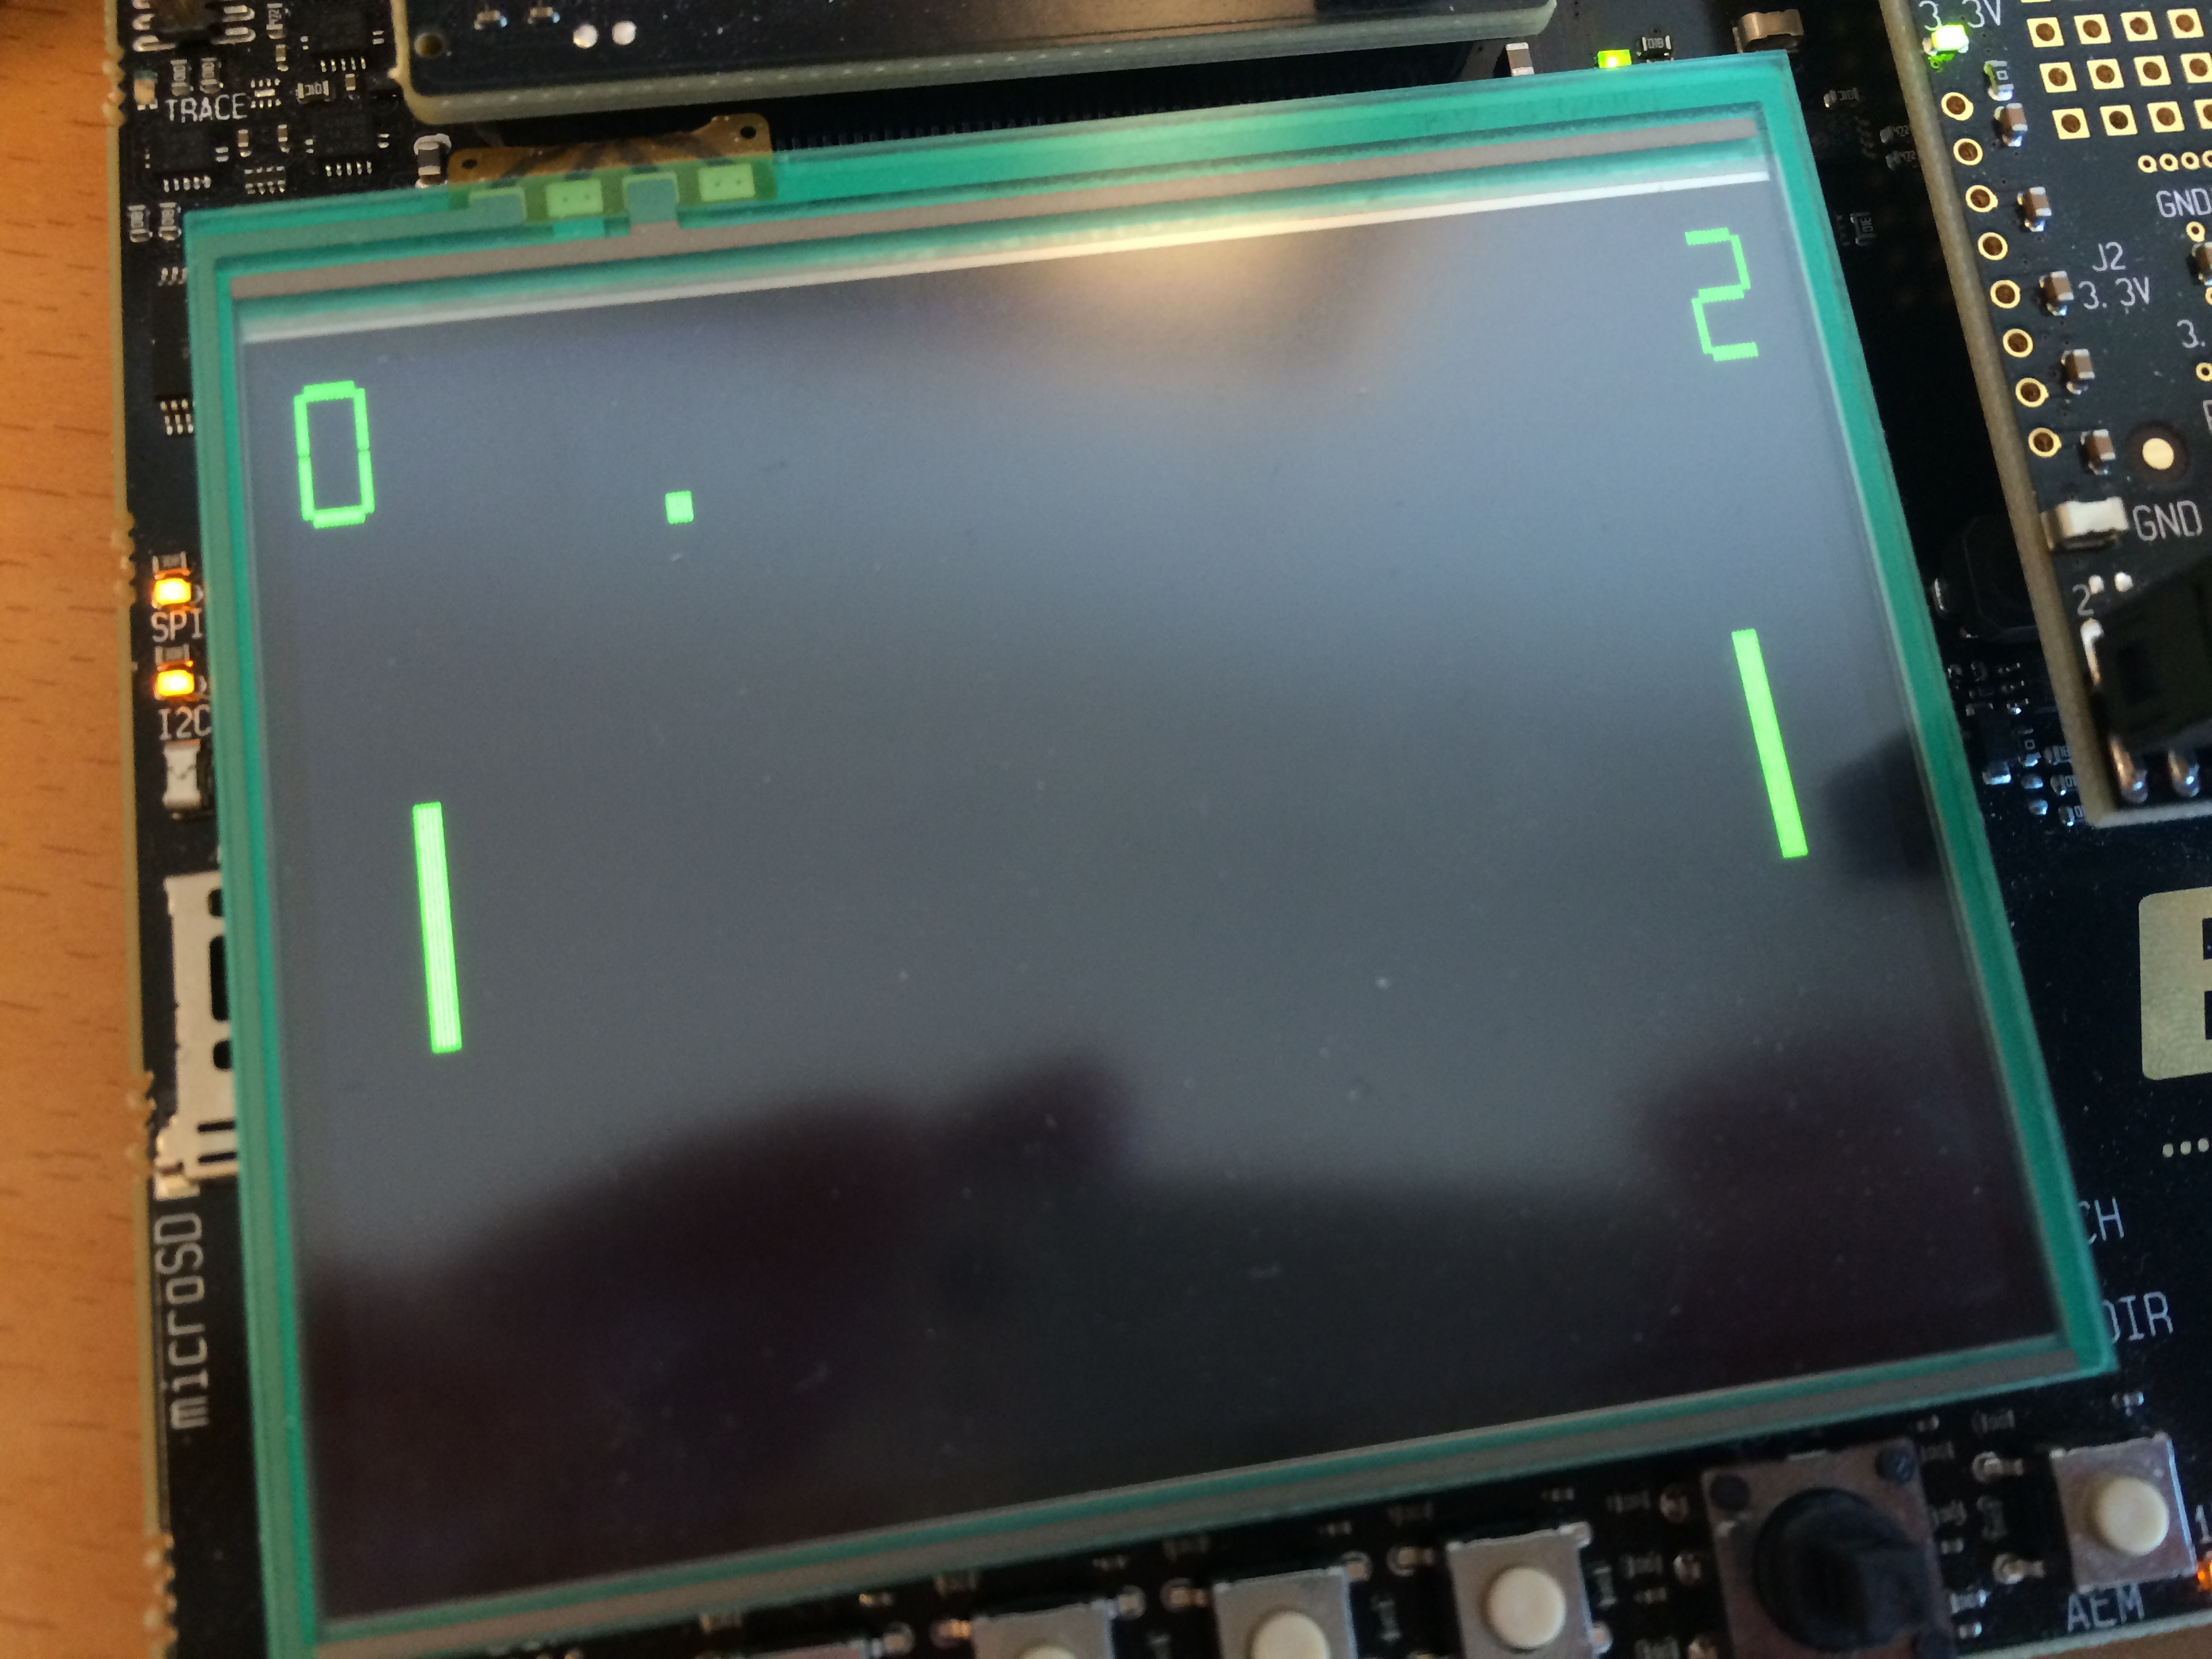
\includegraphics[width=0.8\textwidth]{figures/gameplay.jpg}
\caption{Game play shot}

\end{figure}

\subsubsection{Structure of the game}

Following established patterns of game programming, updates of the games
internal state are fully decoupled from the rendering thereof.

At the start of each iteration of the game loop, lag (how much time we haven't
accounted for) is calculated, and caught up with.
This allows the game to simulate at a fixed rate even on slower hardware,
reducing visual performance only.

If the game loop finishes ahead of time (using less than MS\_PER\_UPDATE ms),
sleep mode is entered for the remainder (time\_to\_next\_update).

The extremely tuned Pong-implementation presented herein spends roughly $ 1 ms
$ in each loop iteration, allowing a maximum framerate of $ 1000 fps $.  When
targeting $ 24 fps $, the program can sleep for $ 41 ms $ per $ 42 ms $ cycle,
spending $ 97 \% $ of execution sleeping.

\begin{algorithm}
  \caption{Game main loop}
  \begin{algorithmic}
    \State $lag \gets 0$
    \State $time\_previous \gets \Call{get\_time}{\null}$

    \Loop
      \State $time\_current \gets \Call{get\_time}{\null}$
      \State $time\_elapsed \gets time\_current - time\_previous$
      \State $lag \gets lag + time\_elapsed$

      \While{$lag \geq MS\_PER\_UPDATE$}
        \State $\Call{update}{\null}$
        \State $lag \gets lag - MS\_PER\_UPDATE$
      \EndWhile
      \State $\Call{draw\_game}{\null}$
      \State $\Call{sleep}{MS\_PER\_UPDATE - lag}$
    \EndLoop
  \end{algorithmic}
\end{algorithm}

\subsubsection{Input handling}
Whenever the gamepad changes state, i.e. a button is released or pressed,
a signal is received which in turn invokes an input interrupt handler.

The handler polls the gamepad driver, receiving a byte representing currently
pressed buttons. Input is then parsed to fit the games internal representation
of active keys. This abstraction layer between input and internal state is used
to allow for multiple methods of input, practical during development when a
computer keyboard is used.

Having an always up to date version of button state cached frees the program
from having to poll the driver for each iteration of the main game loop.

\subsubsection{Graphics}
To display graphics on the screen, the game uses the Linux framebuffer device.
All the functions for initializing and adding graphics to the framebuffer are
contained in graphics.s.

The initializing function opens the framebuffer file in Linux, and then maps
the file to a region in memory. This is done as it is easier to access an array
in memory than to search back and forth in a file.

As a write to the memory mapped area does not update the framebuffer,
one has to refresh it explicitly.
This is done by sending a special signal to the framebuffer
along with bounding indexes, allowing for partial screen updates.

The draw\_pixel() function is used to fill a given pixel with some color.  When
called on a sequence of pixels more complex graphics can be created.  This Pong
implementation includes a fully-functional 7-segment digital watch display,
used for displaying player scores.

To get that nice retro look, all geometry in this implementation of Pong is
rectangular, set to the color of H4CK3R\_GR33N (The Matrix-green).

\subsubsection{Energy efficiency optimization}
After the observation that
roughly $ 99 \% $ of time spent in each iteration of the main game loop (122
out of 123 ms) was consumed inside the render function redrawing the
\emph{entire} framebuffer, it was realized that system calls are a costly
operation and should be kept to a minimum.

To relieve this fact, drawing techniques went through two stages of
improvements, both mandating the inclusion of a previous\_position attribute on
paddles and puck.

The first improvement consists of moving the framebuffer refresh into the
rectangle-rendering function, refreshing only modified parts of the
framebuffer.  The second improvement consists of calculating the difference
between the current and previous positions of game play objects, redrawing only
the difference between them.  This allows for considerable savings as a paddle
at most moves three pixels per frame, allowing a tenfold reduction in system
calls.

The original approach has $ 320 * 240 = 76800 $ system calls per frame,
spending $ 123 ms $ doing so.  The first improvement reduces this to 
$ 240 * 2 * 2+ 25 * 2 = 1010 $ system calls (2 paddles, 1 puck, 1 draw to clear
previous position, 1 to draw new one).  The final system has 
$ 15 * 2 * 2 + 21 * 2 = 102$ system calls (Drawing only differences, 3px 
movement speed), spending only $1 ms $ in the render loop.
